\documentclass[a4paper,12pt]{article}

%%% Работа с русским языком % для pdfLatex
\usepackage{cmap}					% поиск в~PDF
\usepackage{mathtext} 				% русские буквы в~фомулах
\usepackage[T2A]{fontenc}			% кодировка
\usepackage[utf8]{inputenc}			% кодировка исходного текста
\usepackage[english,russian]{babel}	% локализация и переносы
\usepackage{indentfirst} 			% отступ 1 абзаца

%%% Работа с русским языком % для XeLatex
%\usepackage[english,russian]{babel}   %% загружает пакет многоязыковой вёрстки
%\usepackage{fontspec}      %% подготавливает загрузку шрифтов Open Type, True Type и др.
%\defaultfontfeatures{Ligatures={TeX},Renderer=Basic}  %% свойства шрифтов по умолчанию
%\setmainfont[Ligatures={TeX,Historic}]{Times New Roman} %% задаёт основной шрифт документа
%\setsansfont{Comic Sans MS}                    %% задаёт шрифт без засечек
%\setmonofont{Courier New}
%\usepackage{indentfirst}
%\frenchspacing

%%% Дополнительная работа с математикой
\usepackage{amsfonts,amssymb,amsthm,mathtools}
\usepackage{amsmath}
\usepackage{icomma} % "Умная" запятая: $0,2$~--- число, $0, 2$~--- перечисление
\usepackage{upgreek}

%%% Страница
\usepackage{extsizes} % Возможность сделать 14-й шрифт

%% Шрифты
\usepackage{euscript}	 % Шрифт Евклид
\usepackage{mathrsfs} % Красивый матшрифт

%% Свои команды
\DeclareMathOperator{\sgn}{\mathop{sgn}} % создание новой конанды \sgn (типо как \sin)
\usepackage{csquotes} % ещё одна штука для цитат
\newcommand{\pd}[2]{\ensuremath{\cfrac{\partial #1}{\partial #2}}} % частная производная
\newcommand{\abs}[1]{\ensuremath{\left|#1\right|}} % модуль
\renewcommand{\phi}{\ensuremath{\varphi}} % греческая фи
\newcommand{\pogk}[1]{\!\left(\cfrac{\sigma_{#1}}{#1}\right)^{\!\!\!2}\!}

% Ссылки
\usepackage{color} % подключить пакет color
% выбрать цвета
\definecolor{BlueGreen}{RGB}{49,152,255}
\definecolor{Violet}{RGB}{120,80,120}
% назначить цвета при подключении hyperref
\usepackage[unicode, colorlinks, urlcolor=blue, linkcolor=blue, pagecolor=blue, citecolor=blue]{hyperref} %синие ссылки
%\usepackage[unicode, colorlinks, urlcolor=black, linkcolor=black, pagecolor=black, citecolor=black]{hyperref} % для печати (отключить верхний!)
\mathtoolsset{showonlyrefs=true} % Показывать номера только у тех формул, на которые есть \eqref{} в~тексте.


%% Перенос знаков в~формулах (по Львовскому)
\newcommand*{\hm}[1]{#1\nobreak\discretionary{}
	{\hbox{$\mathsurround=0pt #1$}}{}}

%%% Работа с картинками
\usepackage{graphicx}  % Для вставки рисунков
\graphicspath{{images/}{images2/}}  % папки с картинками
\setlength\fboxsep{3pt} % Отступ рамки \fbox{} от рисунка
\setlength\fboxrule{1pt} % Толщина линий рамки \fbox{}
\usepackage{wrapfig} % Обтекание рисунков и таблиц текстом
\usepackage{multicol}

%%% Работа с таблицами
\usepackage{array,tabularx,tabulary,booktabs} % Дополнительная работа с таблицами
\usepackage{longtable}  % Длинные таблицы
\usepackage{multirow} % Слияние строк в~таблице
\usepackage{caption}
\captionsetup{labelsep=period, labelfont=bf}

%%% Оформление
\usepackage{indentfirst} % Красная строка
%\setlength{\parskip}{0.3cm} % отступы между абзацами

%%% Теоремы
\theoremstyle{plain} % Это стиль по умолчанию, его можно не переопределять.
\newtheorem{theorem}{Теорема}[section]
\newtheorem{proposition}[theorem]{Утверждение}

\theoremstyle{definition} % "Определение"
\newtheorem{definition}{Определение}[section]
\newtheorem{corollary}{Следствие}[theorem]
\newtheorem{problem}{Задача}[section]

\theoremstyle{remark} % "Примечание"
\newtheorem*{nonum}{Решение}
\newtheorem{zamech}{Замечание}[theorem]

%%% Правильные мат. символы для русского языка
\renewcommand{\epsilon}{\ensuremath{\varepsilon}}
\renewcommand{\phi}{\ensuremath{\varphi}}
\renewcommand{\kappa}{\ensuremath{\varkappa}}
\renewcommand{\le}{\ensuremath{\leqslant}}
\renewcommand{\leq}{\ensuremath{\leqslant}}
\renewcommand{\ge}{\ensuremath{\geqslant}}
\renewcommand{\geq}{\ensuremath{\geqslant}}
\renewcommand{\emptyset}{\varnothing}

%%% Название разделов
\usepackage{titlesec}
\titlelabel{\thetitle.\quad}

\usepackage{titlesec}
\titleformat{\section}{\normalfont\Large\bfseries}{}{0pt}{}


\title{Laba 4.2.1}
\author{Щадымов Владимир}
\date{April 2018}
\usepackage[left=1.35cm,right=1.35cm,top=1.4cm,bottom=2cm]{geometry}

\begin{document} 

\renewcommand{\figurename}{\textbf{Рис.}}		%Чтобы вместо figure под рисунками писал "рис"
\renewcommand{\tablename}{\textbf{Таблица}}		%Чтобы вместо table над таблицами писал Таблица

\newpage
\begin{titlepage}
\begin{center} 
 
\large Московский физико-технический институт\\
(государственный университет)\\
Факультет молекулярной и химической физики\\
\vspace{32ex}
\huge Лабораторная работа №13\\
\textbf{\Large <<Изучение электронно-колебательных спектров поглощения двухатомных молекул на примере молекулы $I_2$>>}\\
\end{center} 

\vspace{40ex}
{\par \raggedleft \large \emph{Выполнили:}\\ студенты 3 курса\\ 642 группы ФМХФ\\ Шадымов Владимир\\ Георгий Демьянов \par}
\begin{center}
\vfill Москва 2019
\end{center}
\end{titlepage}

\newpage
\pagestyle{plain}
\setcounter{page}{2}

\vspace*{9cm}
\begin{center}
	\vspace{0.5cm}{\parbox{16cm}{\small{\textbf{\centering{Аннотация}\\
					\hspace{0.6cm} В этом отчёте изложены результаты выполнения лабораторной работы
					«Кольца Ньютона».
					В установке кольца Ньютона образуются при интерференции
					световых волн, отражённых от границ тонкой воздушной прослойки,
					заключённой между выпуклой поверхностью линзы и плоской стеклянной пластинкой. Линии постоянной разности хода представляют собой концентрические кольца с центром в точке соприкосновения. Наблюдение ведется в отраженном свете. С помощью микроскопа мы измеряем радиусы темных и светлых колец.
				}}}}
\end{center}


\newpage

\hypersetup{linkcolor=black}
\tableofcontents
\hypersetup{linkcolor=blue}

\newpage
\section{Введение}
\textbf{\emph{Цель работы:}} исследовать явление интерференции на тонких пленках на примере колец Ньютона. Проверить теоретическую зависимость радиуса колец Ньютона от их порядкового номера. Измерить кривизну линзы.

\textbf{\emph{Оборудование:}} измерительный микроскоп с опак-иллюминатором, плосковыпуклая линза, пластинка из черного стекла, ртутная лампа ДРШ-250, щель, линзы, призма прямого зрения, объектная шкала. 
\newpage


\section{Теоретическое введение}

В данном опыте интерференция возникает между лучами, отраженными от нижней пластинки и от кривой поверхности. Геометрическая разность хода между интерферирующими лучами равна удвоенной толщине воздушного зазора $2d$.

\begin{wrapfigure}{r!}{0.3\textwidth}
	\begin{center}
		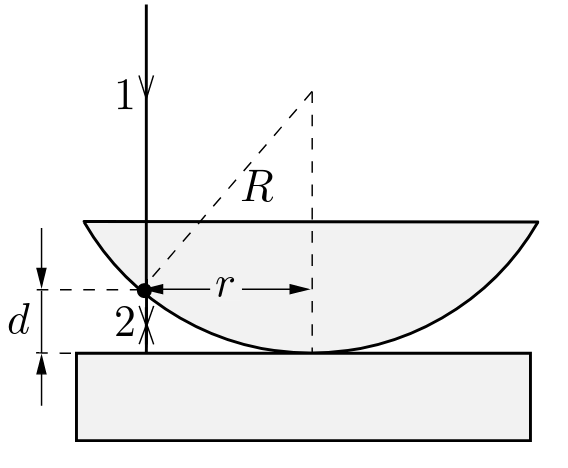
\includegraphics[width=0.25\textwidth,scale=0.35]{theory_pic.png}
		\caption{-- Схема наблюдения колец Ньютона}
		\label{theory_pict}
	\end{center}
	\vspace{5mm}
\end{wrapfigure} 

Для точки на сферической поверхности, находящейся на расстоянии $r$, имеем $r^2 = R^2 -(R-r)^2 = 2Rd-d^2$, где $R$ -- радиус кривизны сферической поверхности (рис. \ref{theory_pict}).


При $R\gg d$ поучим $d=\frac{r^2}{2R}$. С учетом изменения фазы на $\pi$ при отражении волны от оптически более плотной среды получим оптическую разность хода интерферирующих лучей:
\begin{equation}
\Delta = 2d + \frac{\lambda}{2}= \frac{r^2}{R}+\frac{\lambda}{2}.
\end{equation}

\begin{wrapfigure}{r!}{0.3\textwidth}
	\begin{center}
		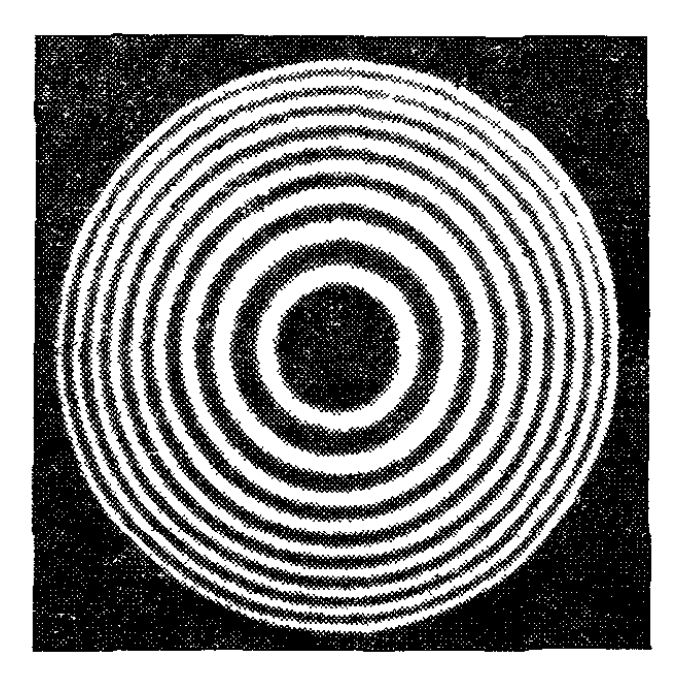
\includegraphics[width=0.2\textwidth,scale=0.2]{circles.png}
		\caption{-- Кольца Ньютона в отраженном свете \cite{Kirichenko}}
		\label{circles}
	\end{center}
\end{wrapfigure}

Условие интерференционного минимума \\ $\Delta=(2m+1)\frac{\lambda}{2};$ $(m=0,1,2,...)$, откуда получаем для радиуса темных колец
\begin{equation}
	r_m=\sqrt{m\lambda R}.
	\label{dark_lines}
\end{equation}

Аналогично для радиусов $r'_m$ светлых колец
\begin{equation}
	r'_m = \sqrt{\frac{(2m-1)\lambda R}{2}}.
	\label{bright_lines}
\end{equation}


Таким образом, в отраженном свете центр колец темный (рис. \ref{circles}).
Заметим, что радиусы колец зависят от длины волны. Поэтому необходимо работать с достаточно узкой частью спектра, выделяя её светофильтрами, или подбирать источник света, который генерирует излучение в узкой части спектра. Последний способ используется в данной работе. Если же свет немонохроматический, то каждое кольцо будет иметь разную окраску в разных его точках. 
\\
\\
\\
\\
\\
%Теоретические выкладки и рисунки взяты из \cite{PrakOptics}~---~c. 91~--~92.


\newpage
\section{Экспериментальная установка}

В эксперименте используется установка, изображенная на рис. \ref{facility}. Источником света служит ртутная лампа. Длины волн ярких линий в спектре ртутной лампы: 
$\lambda_1 = 579,07 нм$ (желтый);   $\lambda_2 = 546,07$ (зеленый). Данные взяты из \cite{PrakOptics}~---~c. 438. Кольца Ньютона в данной работе наблюдаем в желтом цвете.

Пучок света, излучаемый лампой, собирается конденсором \textit{K} в щель \textit{S} и преобразуется коллиматором (щель \textit{S} и объектив \textit{O}) в параллельный пучок. Параллельный пучок разлагается призмой прямого зрения на желтый и зеленый. Желтый свет направляется в опак-иллюминатор \textit{ОИ}. Внутри опак-иллюминатора свет частично отражается от полупрозрачной пластинки \textit{P}, проходит через объектив микроскопа и попадает на линзу. Свет, отраженный от зеркала под линзой, проходит обратно через объектив, полупрозрачную пластинку и окуляр. Так можно наблюдать кольца Ньютона в отраженном свете (рис. \ref{circles}). 
Приборная погрешность измерения шкалы окуляра: $\sigma_{m}=0,03$ мм.
\begin{figure}[h]
	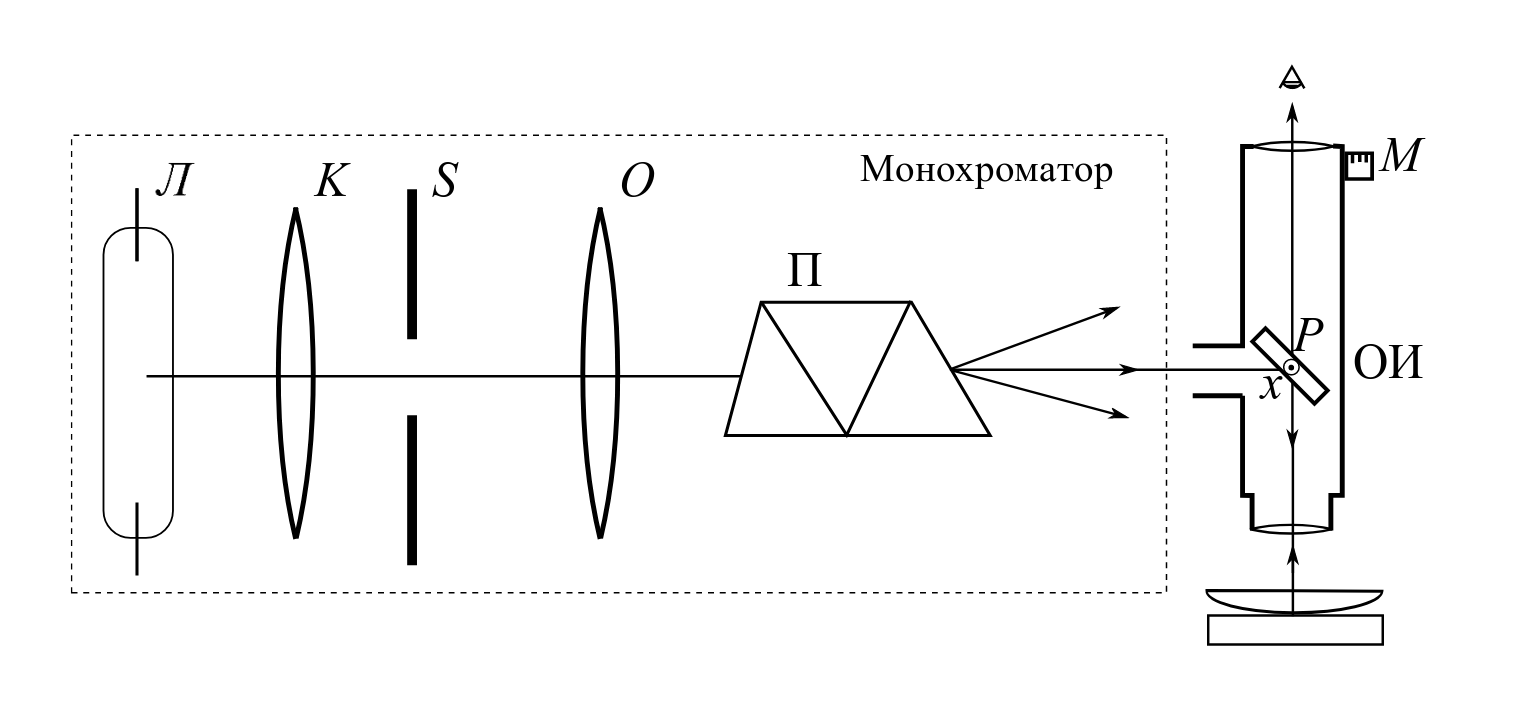
\includegraphics[width=1\textwidth,scale=0.8]{facility_pic.png}
	\caption{Схема установки для наблюдения колец Ньютона: \textit{Л} -- лампа, \textit{K} -- конденсор, \textit{S} -- щель, \textit{П} -- призма прямого зрения, \textit{ОИ} -- опак-иллюминатор, \textit{P} -- полупрозрачная пластинка.}
	\label{facility}
	\vspace{5mm}
\end{figure}

\newpage
\section{Обработка результатов}

Небходимо проверить зависимость $r_m^2(m)$ для темных и светлых колец, где $r_m$ -- радиус кольца порядка $m$.
Приборная погрешность измерения шкалы окуляра: $\sigma_r =3\cdot10^{-2}$ мм\footnote{Так как не было возможности измерить радиус кольца $m$-го порядка несколько раз, для оценки случайной погрешности, то далее при расчетах будем использовать приборную погрешность как полную погрешность радиуса.}.

Измеренные с установки данные занесем в таблицу \ref{table:expdata}.

\begin{table}[h!]
	\centering
	\caption{Экспериментальные данные}
	\label{table:expdata}
	\begin{tabular}{lllll}
		\multicolumn{2}{l}{Темные кольца} &  & \multicolumn{2}{l}{Светлые кольца} \\ \cline{1-2} \cline{4-5} 
		\multicolumn{1}{|l|}{m} & \multicolumn{1}{l|}{$r_m, 10^{-2}$ мм} & \multicolumn{1}{l|}{} & \multicolumn{1}{l|}{m} & \multicolumn{1}{l|}{$r_m, 10^{-2}$ мм} \\ \cline{1-2} \cline{4-5} 
		\multicolumn{1}{|l|}{1} & \multicolumn{1}{l|}{9} & \multicolumn{1}{l|}{} & \multicolumn{1}{l|}{1} & \multicolumn{1}{l|}{7} \\ \cline{1-2} \cline{4-5} 
		\multicolumn{1}{|l|}{2} & \multicolumn{1}{l|}{13} & \multicolumn{1}{l|}{} & \multicolumn{1}{l|}{2} & \multicolumn{1}{l|}{11} \\ \cline{1-2} \cline{4-5} 
		\multicolumn{1}{|l|}{3} & \multicolumn{1}{l|}{15} & \multicolumn{1}{l|}{} & \multicolumn{1}{l|}{3} & \multicolumn{1}{l|}{14} \\ \cline{1-2} \cline{4-5} 
		\multicolumn{1}{|l|}{4} & \multicolumn{1}{l|}{17} & \multicolumn{1}{l|}{} & \multicolumn{1}{l|}{4} & \multicolumn{1}{l|}{16} \\ \cline{1-2} \cline{4-5} 
		\multicolumn{1}{|l|}{5} & \multicolumn{1}{l|}{19} & \multicolumn{1}{l|}{} & \multicolumn{1}{l|}{5} & \multicolumn{1}{l|}{18} \\ \cline{1-2} \cline{4-5} 
		\multicolumn{1}{|l|}{6} & \multicolumn{1}{l|}{20} & \multicolumn{1}{l|}{} & \multicolumn{1}{l|}{6} & \multicolumn{1}{l|}{20} \\ \cline{1-2} \cline{4-5} 
		\multicolumn{1}{|l|}{7} & \multicolumn{1}{l|}{22} & \multicolumn{1}{l|}{} & \multicolumn{1}{l|}{7} & \multicolumn{1}{l|}{21} \\ \cline{1-2} \cline{4-5} 
		\multicolumn{1}{|l|}{8} & \multicolumn{1}{l|}{24} & \multicolumn{1}{l|}{} & \multicolumn{1}{l|}{8} & \multicolumn{1}{l|}{23} \\ \cline{1-2} \cline{4-5} 
	\end{tabular}
\end{table}

Погрешность $r^2_m$ найдем по формуле:
\begin{equation}
	\sigma_{r^2} = \left|\cfrac{\partial r^2_m}{\partial r_m}\right|\sigma_r = 2r_m\sigma_r.
\end{equation}

Пересчитаем данные в удобные для обработки. Полученные результаты занесем в таблицу \ref{table:pre_res}.

\begin{table}[h!]
	\centering
	\caption{Обработанные результаты}
	\label{table:pre_res}
	\begin{tabular}{lllllll}
		\multicolumn{3}{l}{Темные кольца} &  & \multicolumn{3}{l}{Светлые кольца} \\ \cline{1-3} \cline{5-7} 
		\multicolumn{1}{|l|}{m} & \multicolumn{1}{l|}{$r^2_m, 10^{-3}$ мм$^2$} & \multicolumn{1}{l|}{$\sigma_{r^2}, 10^{-3}$ мм$^2$} & \multicolumn{1}{l|}{} & \multicolumn{1}{l|}{m} & \multicolumn{1}{l|}{$r^2_m, 10^{-3}$ мм$^2$} & \multicolumn{1}{l|}{$\sigma_{r^2}, 10^{-3}$ мм$^2$} \\ \cline{1-3} \cline{5-7} 
		\multicolumn{1}{|l|}{1} & \multicolumn{1}{l|}{8} & \multicolumn{1}{l|}{2} & \multicolumn{1}{l|}{} & \multicolumn{1}{l|}{1} & \multicolumn{1}{l|}{5} & \multicolumn{1}{l|}{1} \\ \cline{1-3} \cline{5-7} 
		\multicolumn{1}{|l|}{2} & \multicolumn{1}{l|}{16} & \multicolumn{1}{l|}{3} & \multicolumn{1}{l|}{} & \multicolumn{1}{l|}{2} & \multicolumn{1}{l|}{11} & \multicolumn{1}{l|}{2} \\ \cline{1-3} \cline{5-7} 
		\multicolumn{1}{|l|}{3} & \multicolumn{1}{l|}{22} & \multicolumn{1}{l|}{3} & \multicolumn{1}{l|}{} & \multicolumn{1}{l|}{3} & \multicolumn{1}{l|}{19} & \multicolumn{1}{l|}{3} \\ \cline{1-3} \cline{5-7} 
		\multicolumn{1}{|l|}{4} & \multicolumn{1}{l|}{29} & \multicolumn{1}{l|}{3} & \multicolumn{1}{l|}{} & \multicolumn{1}{l|}{4} & \multicolumn{1}{l|}{24} & \multicolumn{1}{l|}{3} \\ \cline{1-3} \cline{5-7} 
		\multicolumn{1}{|l|}{5} & \multicolumn{1}{l|}{35} & \multicolumn{1}{l|}{4} & \multicolumn{1}{l|}{} & \multicolumn{1}{l|}{5} & \multicolumn{1}{l|}{32} & \multicolumn{1}{l|}{4} \\ \cline{1-3} \cline{5-7} 
		\multicolumn{1}{|l|}{6} & \multicolumn{1}{l|}{42} & \multicolumn{1}{l|}{4} & \multicolumn{1}{l|}{} & \multicolumn{1}{l|}{6} & \multicolumn{1}{l|}{39} & \multicolumn{1}{l|}{4} \\ \cline{1-3} \cline{5-7} 
		\multicolumn{1}{|l|}{7} & \multicolumn{1}{l|}{49} & \multicolumn{1}{l|}{4} & \multicolumn{1}{l|}{} & \multicolumn{1}{l|}{7} & \multicolumn{1}{l|}{45} & \multicolumn{1}{l|}{4} \\ \cline{1-3} \cline{5-7} 
		\multicolumn{1}{|l|}{8} & \multicolumn{1}{l|}{58} & \multicolumn{1}{l|}{5} & \multicolumn{1}{l|}{} & \multicolumn{1}{l|}{8} & \multicolumn{1}{l|}{52} & \multicolumn{1}{l|}{5} \\ \cline{1-3} \cline{5-7} 
	\end{tabular}
\end{table}

Согласно теории (формулы \eqref{dark_lines} и \eqref{bright_lines}) квадрат радиуса кольца $r^2_m$ линейно зависит от его номера $m$. Оценим\footnote{Расчеты коэффициентов проводились с помощью библиотеки \hyperref{https://docs.scipy.org/doc/scipy-0.14.0/reference/generated/scipy.stats.pearsonr.html}{}{}{Scipy}.} эту зависимость через коэффициент корреляции Пирсона.
\begin{itemize}
	\item Для темных колец: $\rho_{dark}=0,9991$; уровень значимости $p<1\%$.
	\item Для светлых колец: $\rho_{light}=0,9994$; уровень значимости $p<1\%$.
\end{itemize}

Видно, что данные сильно коррелируют. Построим\footnote{Графики построены с помощью библиотеки \hyperref{https://matplotlib.org/}{}{}{Matplotlib}.} графики зависимостей $r^2_m(m)$ для темных и светлых колец (рис. \ref{graph}). Проведем\footnote{Регрессия методом наименьших квадратов вычислена с помощью библиотеки \hyperref{http://www.statsmodels.org}{}{}{Statsmodels}.} МНК для этих зависимостей. Согласно теории необходимо наложить некоторые ограничения на регрессию. Для темных колец проводим МНК через точку $r^2_m=0$, $m=0$ \eqref{dark_lines}; для светлых --  $r^2_m=0$, $m=\frac{1}{2}$ \eqref{bright_lines}. 

\begin{itemize}
	\item Из МНК для темных колец по формуле \eqref{dark_lines}: $\lambda R_1=(7,15\pm0,09)\cdot10^{-3}$ мм$^2$.
	\item Из МНК для светлых колец по формуле \eqref{bright_lines}:  $\lambda R_2=(6,99\pm0,08)\cdot10^{-3}$ мм$^2$.
\end{itemize}

Сделаем проверку на выбросы, считая статистику для критерия Стьюдента следующим образом:
\begin{equation}
	S_m = \frac{r^2_m-\mu_0}{\sigma_{r^2_m}/\sqrt{n}} \thicksim t(n_\Sigma-2),
	\label{stats}
\end{equation}
где $r^2_m$ -- квадрат радиус $m$-го кольца; $\mu_0$ -- значение регрессии в данной точке; $\sigma_{r^2_m}$ -- среднеквадратичное отклонение в данной точке, ошибка; $n$ -- число измерений в данной точке, в данном случае равно $1$; $n_\Sigma$ -- полное число измерений, в данном случае равно $8$. Есть два зависимых параметра (степени свободы): коэффициент регрессии МНК через фиксированную точку, оценочное среднеквадратичное отклонение.  Соответствующие уровни значимости\footnote{Расчеты уровней значимости проводились с помощью библиотеки \hyperref{https://docs.scipy.org/doc/scipy/reference/generated/scipy.stats.t.html}{}{}{Scipy}.} занесем в таблицу \ref{pvalue}. Считаем критический уровень значимости 5\%.

\begin{figure}[h!]
	\noindent\centering{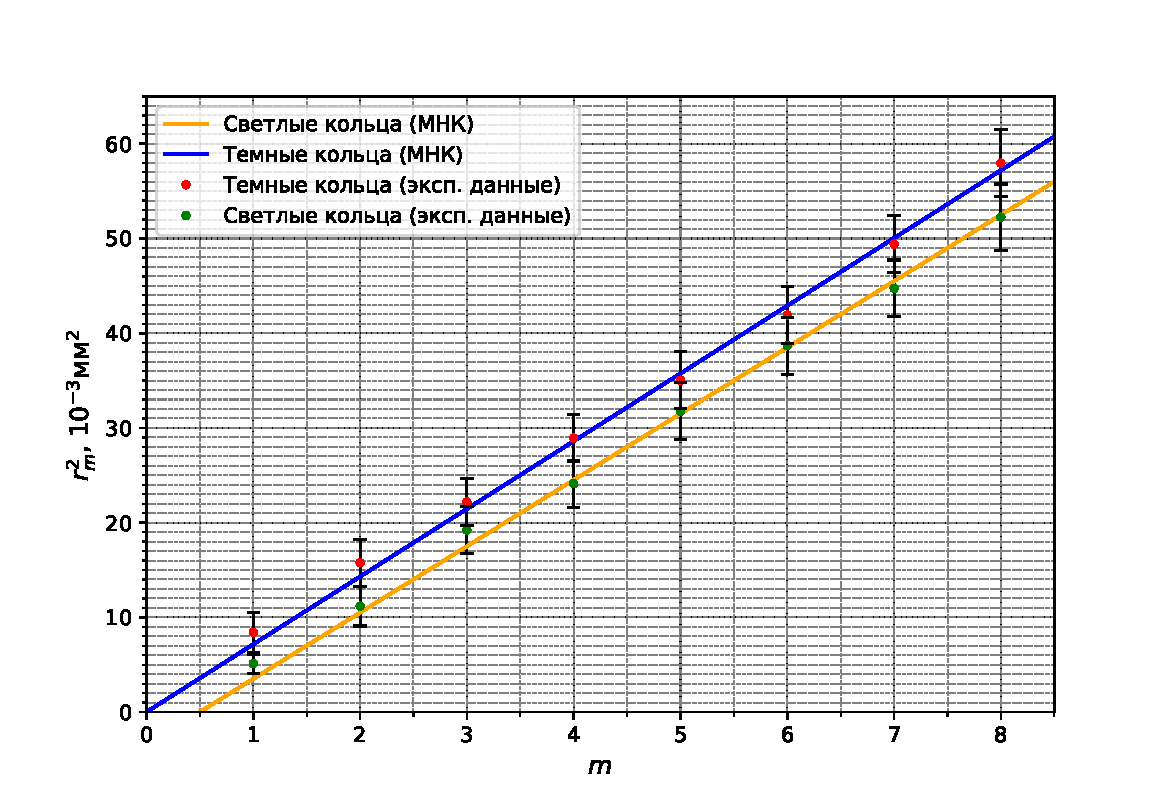
\includegraphics[width=19cm]{colored_graph.pdf}}
	\vspace{-0.5cm}
	\caption{ Зависимость квадрата радиуса колец $r^2_m(m)$ от порядкового номера $m$.}
	\label{graph}
\end{figure}

\begin{table}[h!]
	\centering
	\caption{Значения статистик и уровней значимости}
	\label{pvalue}
	\begin{tabular}{lllllllllll}
		\multicolumn{5}{l}{Темные кольца} &  & \multicolumn{5}{l}{Светлые кольца} \\ \cline{1-5} \cline{7-11} 
		\multicolumn{1}{|l|}{m} & \multicolumn{1}{l|}{$r^2_m, 10^{-3}$ мм$^2$} & \multicolumn{1}{l|}{$S_m$} & \multicolumn{1}{l|}{$p$-$value$} & \multicolumn{1}{l|}{Итог} & \multicolumn{1}{l|}{} & \multicolumn{1}{l|}{m} & \multicolumn{1}{l|}{$r^2_m, 10^{-3}$ мм$^2$} & \multicolumn{1}{l|}{$S_m$} & \multicolumn{1}{l|}{$p$-$value$} & \multicolumn{1}{l|}{Итог} \\ \cline{1-5} \cline{7-11} 
		\multicolumn{1}{|l|}{1} & \multicolumn{1}{l|}{8} & \multicolumn{1}{l|}{0,696} & \multicolumn{1}{l|}{0,256} & \multicolumn{1}{l|}{Не выброс} & \multicolumn{1}{l|}{} & \multicolumn{1}{l|}{1} & \multicolumn{1}{l|}{5} & \multicolumn{1}{l|}{1,020} & \multicolumn{1}{l|}{0,174} & \multicolumn{1}{l|}{Не выброс} \\ \cline{1-5} \cline{7-11} 
		\multicolumn{1}{|l|}{2} & \multicolumn{1}{l|}{16} & \multicolumn{1}{l|}{0,583} & \multicolumn{1}{l|}{0,291} & \multicolumn{1}{l|}{Не выброс} & \multicolumn{1}{l|}{} & \multicolumn{1}{l|}{2} & \multicolumn{1}{l|}{11} & \multicolumn{1}{l|}{0,176} & \multicolumn{1}{l|}{0,433} & \multicolumn{1}{l|}{Не выброс} \\ \cline{1-5} \cline{7-11} 
		\multicolumn{1}{|l|}{3} & \multicolumn{1}{l|}{22} & \multicolumn{1}{l|}{0,247} & \multicolumn{1}{l|}{0,407} & \multicolumn{1}{l|}{Не выброс} & \multicolumn{1}{l|}{} & \multicolumn{1}{l|}{3} & \multicolumn{1}{l|}{19} & \multicolumn{1}{l|}{0,451} & \multicolumn{1}{l|}{0,334} & \multicolumn{1}{l|}{Не выброс} \\ \cline{1-5} \cline{7-11} 
		\multicolumn{1}{|l|}{4} & \multicolumn{1}{l|}{29} & \multicolumn{1}{l|}{0,098} & \multicolumn{1}{l|}{0,462} & \multicolumn{1}{l|}{Не выброс} & \multicolumn{1}{l|}{} & \multicolumn{1}{l|}{4} & \multicolumn{1}{l|}{24} & \multicolumn{1}{l|}{0,324} & \multicolumn{1}{l|}{0,378} & \multicolumn{1}{l|}{Не выброс} \\ \cline{1-5} \cline{7-11} 
		\multicolumn{1}{|l|}{5} & \multicolumn{1}{l|}{35} & \multicolumn{1}{l|}{0,189} & \multicolumn{1}{l|}{0,428} & \multicolumn{1}{l|}{Не выброс} & \multicolumn{1}{l|}{} & \multicolumn{1}{l|}{5} & \multicolumn{1}{l|}{32} & \multicolumn{1}{l|}{0,142} & \multicolumn{1}{l|}{0,446} & \multicolumn{1}{l|}{Не выброс} \\ \cline{1-5} \cline{7-11} 
		\multicolumn{1}{|l|}{6} & \multicolumn{1}{l|}{42} & \multicolumn{1}{l|}{0,239} & \multicolumn{1}{l|}{0,410} & \multicolumn{1}{l|}{Не выброс} & \multicolumn{1}{l|}{} & \multicolumn{1}{l|}{6} & \multicolumn{1}{l|}{39} & \multicolumn{1}{l|}{0,188} & \multicolumn{1}{l|}{0,429} & \multicolumn{1}{l|}{Не выброс} \\ \cline{1-5} \cline{7-11} 
		\multicolumn{1}{|l|}{7} & \multicolumn{1}{l|}{49} & \multicolumn{1}{l|}{0,142} & \multicolumn{1}{l|}{0,446} & \multicolumn{1}{l|}{Не выброс} & \multicolumn{1}{l|}{} & \multicolumn{1}{l|}{7} & \multicolumn{1}{l|}{45} & \multicolumn{1}{l|}{0,432} & \multicolumn{1}{l|}{0,340} & \multicolumn{1}{l|}{Не выброс} \\ \cline{1-5} \cline{7-11} 
		\multicolumn{1}{|l|}{8} & \multicolumn{1}{l|}{58} & \multicolumn{1}{l|}{0,158} & \multicolumn{1}{l|}{0,440} & \multicolumn{1}{l|}{Не выброс} & \multicolumn{1}{l|}{} & \multicolumn{1}{l|}{8} & \multicolumn{1}{l|}{52} & \multicolumn{1}{l|}{0,318} & \multicolumn{1}{l|}{0,381} & \multicolumn{1}{l|}{Не выброс} \\ \cline{1-5} \cline{7-11}   
	\end{tabular}
\end{table}



Таким образом, выбросов не оказалось. Вычислим радиус кривизны линзы.
\begin{equation}
	R = \frac{R_1+R_2}{2}.
\end{equation}

Соответствующая погрешность:

\begin{equation}
	\sigma_R = \sqrt{\sigma_{Rrand}^2+\sigma_{Rindirect}^2} . 
\end{equation}

Получаем $R = (1,22\pm0,03)$ см. Значение со среднеквадратичным отклонением.

Так как было два измерения радиуса, то доверительному интервалу с вероятностью 0,95, соответствует коэффициент Cтьюдента $t(1-0,95;2)=4,3$. Итоговое значение радиуса с вероятностью $0,95$ находится в интервале: $R = (1,22\pm0,12)$ см. 

%\begin{itemize}
%	\item В процессе опыта происходили как колебания маятников, так и колебания струны перпендикулярно столу (проще говоря "вверх-вниз").
%	\item Условие равенства длин AC, CD, DB не было соблюдено.
%	\item Возможные ошибки при подготовке установки к проведению опыта.
%\end{itemize}
\newpage
\section{Заключение}
\begin{itemize}
	\item Данный эксперимент с достаточно высокой точностью подтверждает теоретическую зависимость радиуса колец Ньютона от их порядкового номера $r_m(m)$. Уровни значимости корреляции  $p<1\%$.
	\item Радиус кривизны линзы: $R=(1,22\pm0,12)$ см. Относительная ошибка $\epsilon=9,8\%$.
\end{itemize} 

\bibliography{mybibliography}
\bibliographystyle{gost705}




\end{document}